\section{Discussion} \label{sec:discussion}

In this section, we examine current and previous DNS-based and other
cryptographic schemes, most of which are based on public key cryptography.
Further, we note PGP's limiting human factors, how those factors also apply to
the checksum solution, and how the \SYSTEM{} solution avoids them. Thereafter,
we discuss some limitations of the \SYSTEM{} methodology, implementation, and
DNS itself.

\subsection{Additional Related Work}

\noindent\textbf{Cryptographic Data in DNS Resource Records.} Storing
cryptographic data in the DNS network is not a new idea. The DNS-Based
Authentication of Named Entities (DANE) specification~\cite{DANE1, DANE2, DANE3}
defines the ``TLSA'' and ``OPENPGPKEY'' DNS resource records to store
cryptographic data. These resource record types, along with
``CERT''~\cite{CERT}, ``IPSECKEY''~\cite{IPSECKEY}, those defined by DNS
Security Extensions (DNSSEC)~\cite{DNSSEC}, and others demonstrate that storing
useful cryptographic data retrievable through the DNS network is feasible at
scale. With \SYSTEM{}, however, we use ``TXT'' records to map Resource
Identifiers to Authoritative Hashes. In accordance with RFC 5507~\cite{RFC5507},
an actual \SYSTEM{} implementation would necessitate the creation of a new DNS
resource record type. \\

\noindent\textbf{PGP/OpenPGP.} Though PGP addresses a fundamentally different
threat model than \SYSTEM{}, it is useful to note: many of the same human and UX
factors that make the cryptographically solid OpenPGP standard and its various
implementations so unpleasant for end users also exist in the context of
download integrity verification and checksums. End users cannot and \textit{will
not} be burdened with manually verifying a checksum; as was the case with PGP
5.0~\cite{PGPBad}, some users are likely confused by the very notion of a
checksum, if they are aware of checksums at all. If PGP's adoption issues are
any indication, users of a security solution that significantly complicate an
otherwise simple task are more likely to bypass said solution rather than be
burdened with it. To assume otherwise can have disastrous
consequences~\cite{PGPBad} (also see: \secref{background}). \\

\noindent\textbf{Link Fingerprints and Subresource Integrity.} The Link
Fingerprints (LF) draft describes an early HTML anchor and URL based resource
integrity verification scheme~\cite{LF}. Subresource Integrity (SRI) describes a
similar production-ready HTML-based scheme designed with CDNs in mind. Like
\SYSTEM{}, both LF and SRI employ cryptographic digests to ensure no changes of
any kind have been made to a resource file~\cite{SRI}. Unlike \SYSTEM{}, LF and
SRI rely on the server that hosts the HTML source to be secure; specifically,
the checksums contained in the HTML source must be accurate for these schemes to
work. An attacker that has control of the web server can alter the HTML and
inject a malicious checksum. With \SYSTEM{}, however, an attacker would also
have to compromise the DNS zone or whichever distributed system hosted the
mappings between Resource Identifers and Authoritative Hashes. \\

\noindent\textbf{Content-MD5 Header.} The Content-MD5 header field is a
deprecated email and HTTP header that delivers a checksum similar to those used
by Subresource Integrity. It was removed from the HTTP/1.1 specification because
of the inconsistent implementation of partial response handling between
vendors~\cite{HTTP1.1}. Further, the header could be easily stripped off or
modified by proxies and other intermediaries~\cite{MD5Header}. \\

\noindent\textbf{Code Signing.} \TODO{(I think we should address the differences
explicitly: we're simpler; we don't make the system more fragile; no central
authority; applicable to more than just software binaries)}

\subsection{Limitations}

\subsubsection{DNSSEC Adoption is Slow}

DNSSEC is hard to configure correctly~\cite{DNSSEC-is-hard-1, DNSSEC-is-hard-2,
DNSSEC-is-hard-3, DNSSEC-is-hard-4}, which make services that attempt to deploy
it significantly more \textit{fragile}. For instance, services deploying DNSSEC
become vulnerable to small DNSSEC resource record misconfigurations that can
take entire services offline with varying levels of conspicuousness. Further,
any DNS-related issue becomes harder to diagnose with DNSSEC enabled. Some
registrars and DNS operators do not offer DNSSEC capability at all, restrict
access behind a paywall, or lack an interface for proper key
management~\cite{Cloudflare}. Despite ongoing efforts to simply DNSSEC
deployment, adoption remains low for these reasons. Only around 3\% of Fortune
1000 and 9\% of university domains, a number that is very slowly on the
rise~\cite{NIST}.

On the client side, adoption of DNSSEC validation by DNS resolvers is low and
growth is slow. \figref{apnic} shows that, worldwide, some 14\% of DNS requests
have DNSSEC extensions validated by the resolver towards the end of
2018~\cite{APNIC}. The overall trend is positive thanks to large public
resolvers like Google (8.8.8.8 and 8.8.4.4) and Cloudflare/APNIC (1.1.1.1), as
well as the increasing number of compliant local/ISP resolvers.

\begin{figure}[t]
    \centering
    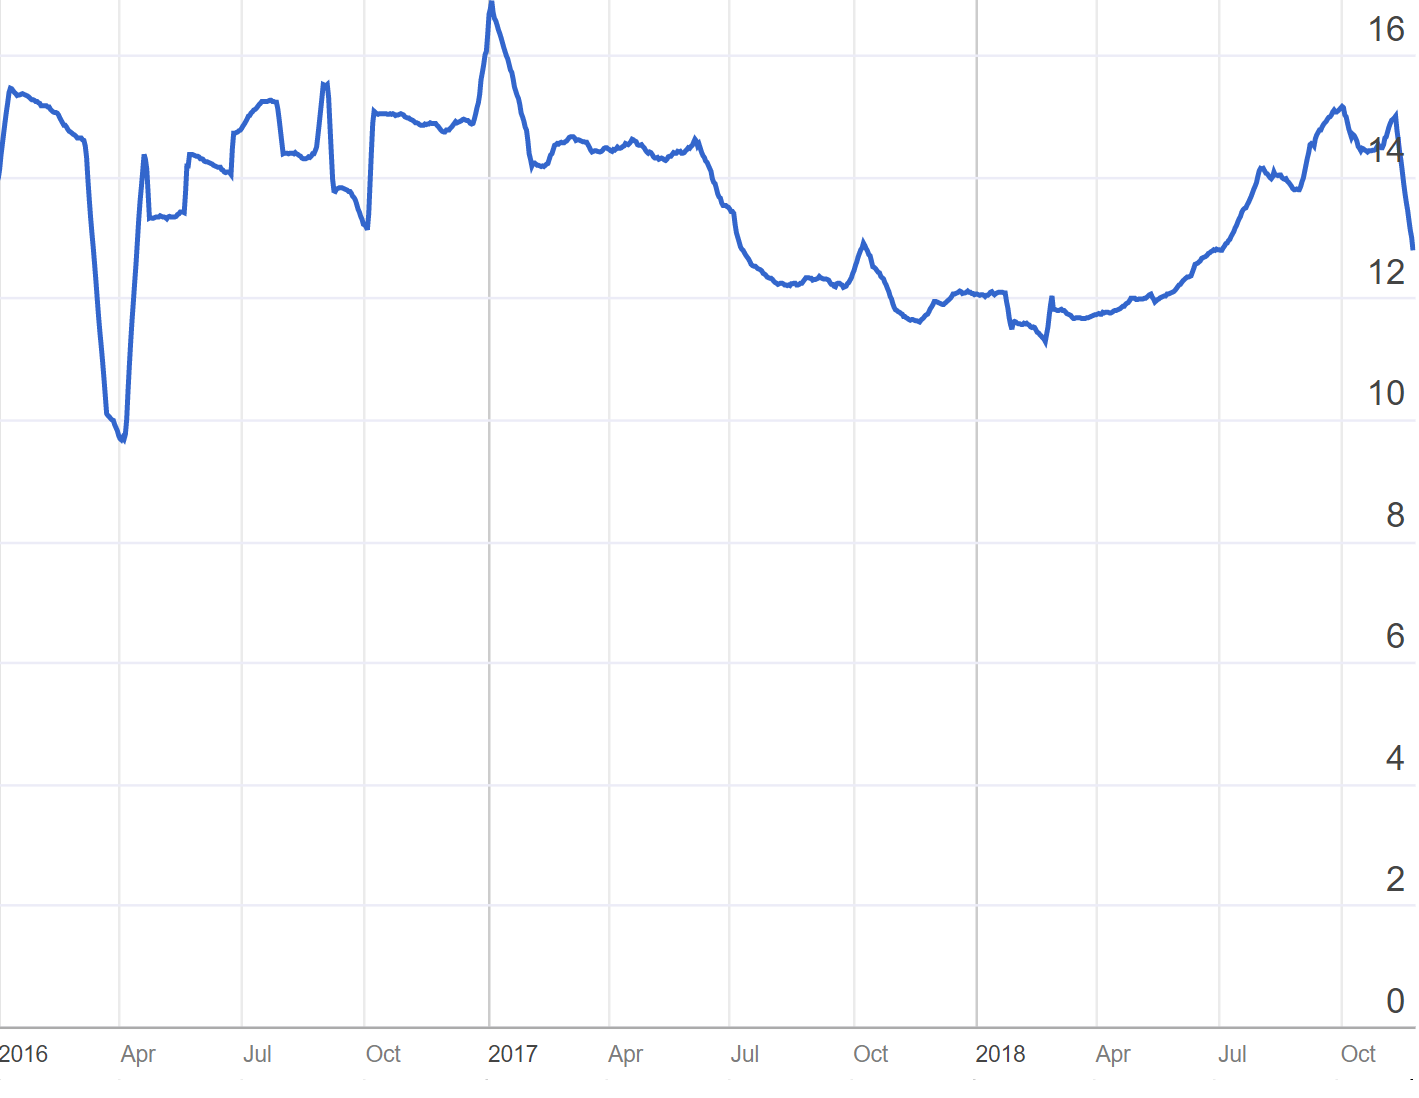
\includegraphics[width=0.95\linewidth]{apnic.png}
    \caption{APNIC estimate of global DNS resolvers (Google PDNS as well as
    local resolvers) performing DNSSEC validation from January 2016 to December
    2018.}\label{fig:apnic}
\end{figure}

It should be noted that DNSSEC does not necessarily make the DNS network, i.e.
properly configured DNS servers, more vulnerable to amplification or other types
of reflection attacks~\cite{Ariya} than it already is as a UDP-based content
delivery service~\cite{USCERT, Vixie}.

\subsubsection{DNS-Specific Protocol Limitations}

DNS~\cite{DNS1} was not originally designed to transport or store relatively
large amounts of data, though this has been addressed with EDNS0~\cite{EDNS}.
The checksums stored in DNS shouldn't be much longer than 128 bytes or the
output of the SHA512 function. Regardless, DNS resource record extensions exist
that store much more than 128 bytes of data~\cite{CERT, IPSECKEY, DANE3, DANE1}.

Several working groups are considering DNS as a storage medium for
checksums/hash output as well, such as securitytxt~\cite{draft-sectxt}. A widely
deployed example of DNS ``TXT'' resource records being used this way is SPF and
DKIM~\cite{DKIM}.

Additionally, \SYSTEM{} does not add to the danger of amplification and other
reflection attacks on DNS; these are generic DNS issues addressable at other
layers of the protocol.

\subsubsection{Supply Chain Attack Diversity}

\TODO{There are many types of SCAs that can occur at any phase of the software
development life cycle. \SYSTEM{} only protects against attacks in the latter 3
categories. (Maybe bring the table back?) (Maybe talk about CCleaner falling out
of scope?)}

\subsubsection{Chrome Implementation}

Our current JavaScript proof-of-concept implementation, as a Chrome extension,
isn't allowed to touch the resource file downloaded by Chrome and so can't
prevent the potentially-malicious resource file from being executed by the end
user—a feature Chrome/Chromium reserves for its own internal use. The Chrome
\textit{app} API~\cite{AppAPI} might have been of assistance as it allowed for
some limited filesystem traversal via a now deprecated native app API; there is
also a non-standard HTML5/WebExtensions FileSystem API that would provide
similar functionality were it to be widely considered~\cite{deadSpec}.

\SYSTEM{} would be even more effective as a browser extension if Chrome/Chromium
or the WebExtensions API allowed for an explicit \texttt{onComplete} event hook
in the downloads API. This hook would fire immediately before a file download
completed and the file became executable, \ie had its \texttt{.crdownload} or
\texttt{.download} extension removed. The hook would consume a
\texttt{Promise}/\texttt{AsyncFunction} that kept the download in its
non-complete state until said \texttt{Promise} completed. This would allow
\SYSTEM{}'s background page to do something like alter the download's
\texttt{DangerType} property and alert the end user to the dangerous download
naturally. This would have the advantage of communicating intent through the
browser's familiar UI and preventing the potentially-malicious download from
becoming immediately executable. Unfortunately, the closest the
Chrome/WebExtensions API comes to allowing \texttt{DangerType} mutations is the
\texttt{acceptDanger} method on the downloads API, but it is not suitable for
use with \SYSTEM{} as a background page based extension.

\subsection{Future Work}

\subsubsection{Merkle Trees and Early Resource Validation}

Using Merkle Trees instead of pure hashing functions to offer partial
verification of large files, i.e. if the file we're downloading is 10TiB, we
don't have to wait for it to finish downloading before we render a failing
judgement. This saves the user time. Perhaps using the Tiger hash, since Tiger
Merkle Trees seem to be popular among large P2P and file sharing applications.

\subsubsection{Replacing RIs with URNs}

The goal of the Resource Identifiers (RI) is very similar to that of Uniform
Resource Names (URN). It may make sense to replace the mapping between RIs and
Authoritative Hashes with purely URN-based DNS lookups that return specially
formatted TXT records upon success. This would further simplify the deployment
process for service administrators since DNS updates would be based upon the
resource's contents instead of both its contents \textit{and where it is located
physically on a distribution server}. It may also allow for additional
confirmation methods of the identical resources in different domains and in
different locations.

We did not choose a URN-based scheme in our initial approach due to a new URN
scheme requiring the registration of a unique identifier with the Internet
Assigned Numbers Authority. Going forward, we can potentially adopt a URN scheme
that already exists, such as Magnet links~\cite{MagnetLinks} or the informal
IETF draft for hash-based URN namespaces~\cite{draft-URN}. With URNs, we can
ensure our naming scheme is based solely on a resource's contents rather than
both its contents and it's location on a web server.
